%-----------------------------------------------------------------------------------------------------------------
\chapter{Introduction}
\label{Ch:Introducao}
%---------------------------------------------------------------------------------------------------------------

\section{Context}

\sloppy %to force margin indentation
The robotic grasping is an important and challenging task that is still today the focus of several research works. Although this function is intuitive and mastered by humans, for robots, it is a contemporary and imperative issue. The range of applications is wide, e.g., from bin-picking in the industry's logistics to a delicate and accurate human-machine interaction in domestic and collaborative robots applications.


\begin{figure}[h!]
\resizebox{1\textwidth}{!}{%
\begin{tcolorbox}
     \centering
     \begin{subfigure}[c]{0.45\textwidth}
         \centering
         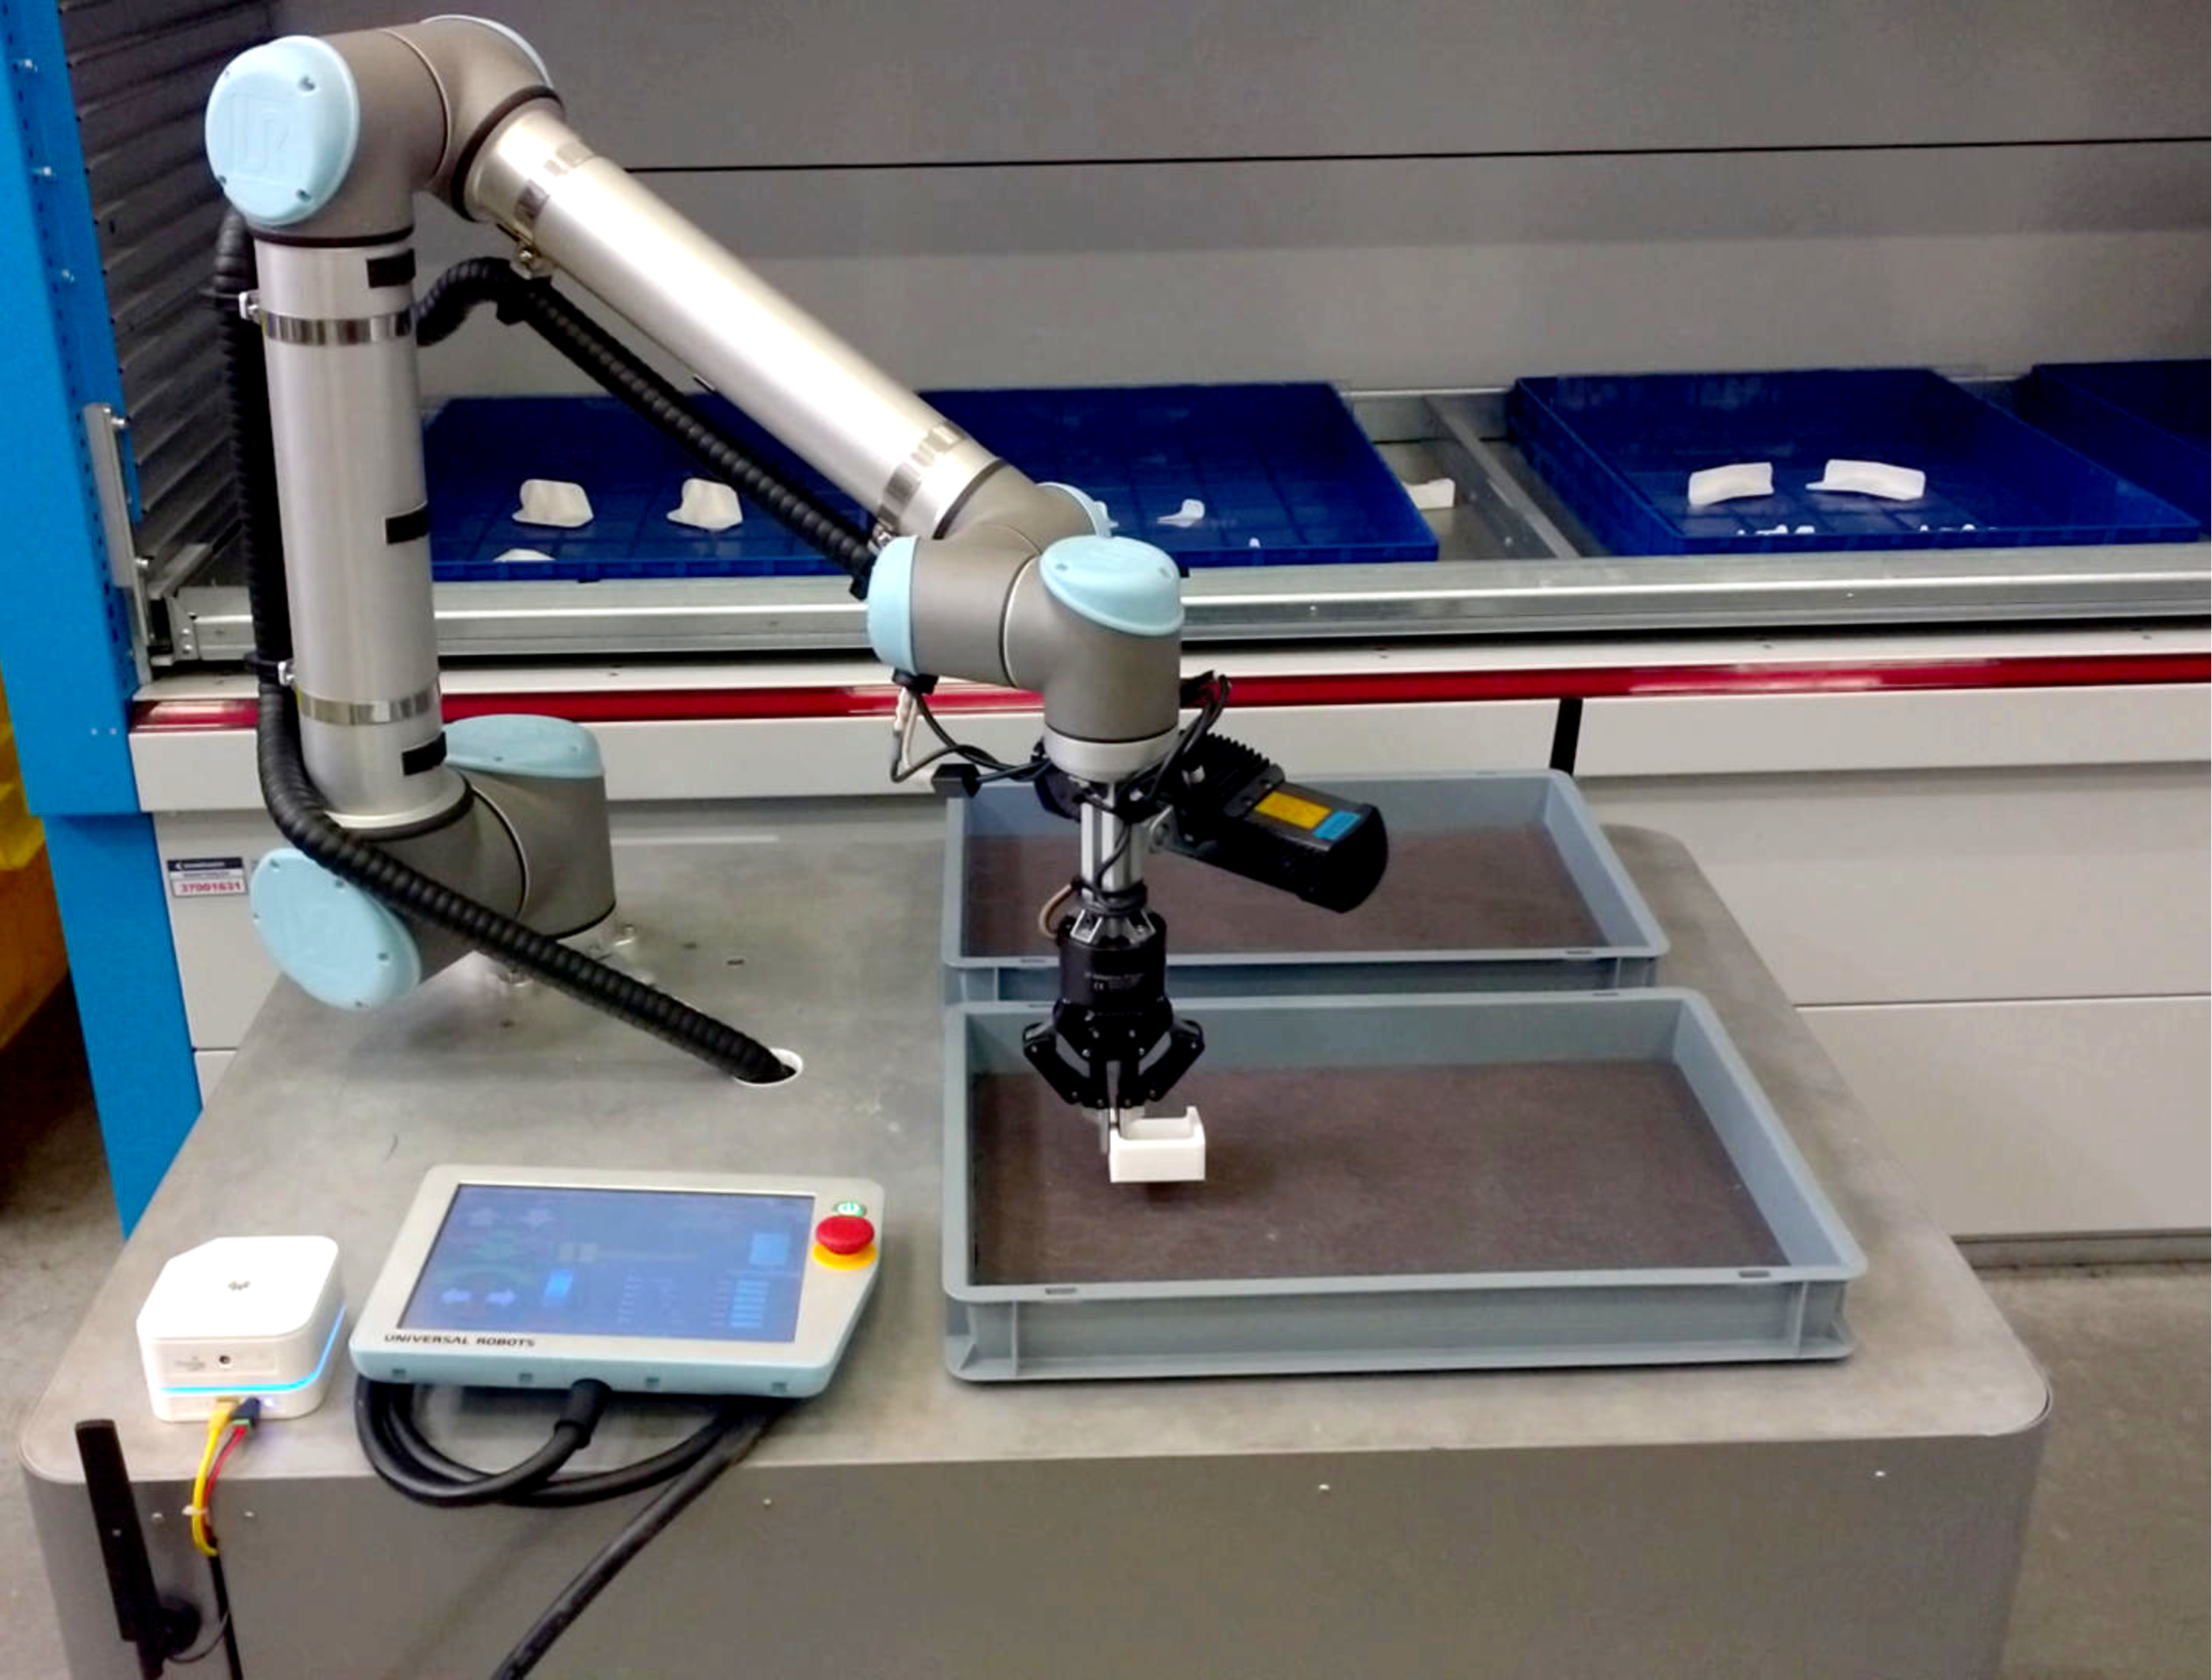
\includegraphics[width=1\textwidth]{Cap1/Figuras/platform.pdf}
         \caption{Industrial application.}
         \label{fig:g1}
     \end{subfigure}
     \hfill
     \begin{subfigure}[c]{0.45\textwidth}
         \centering
         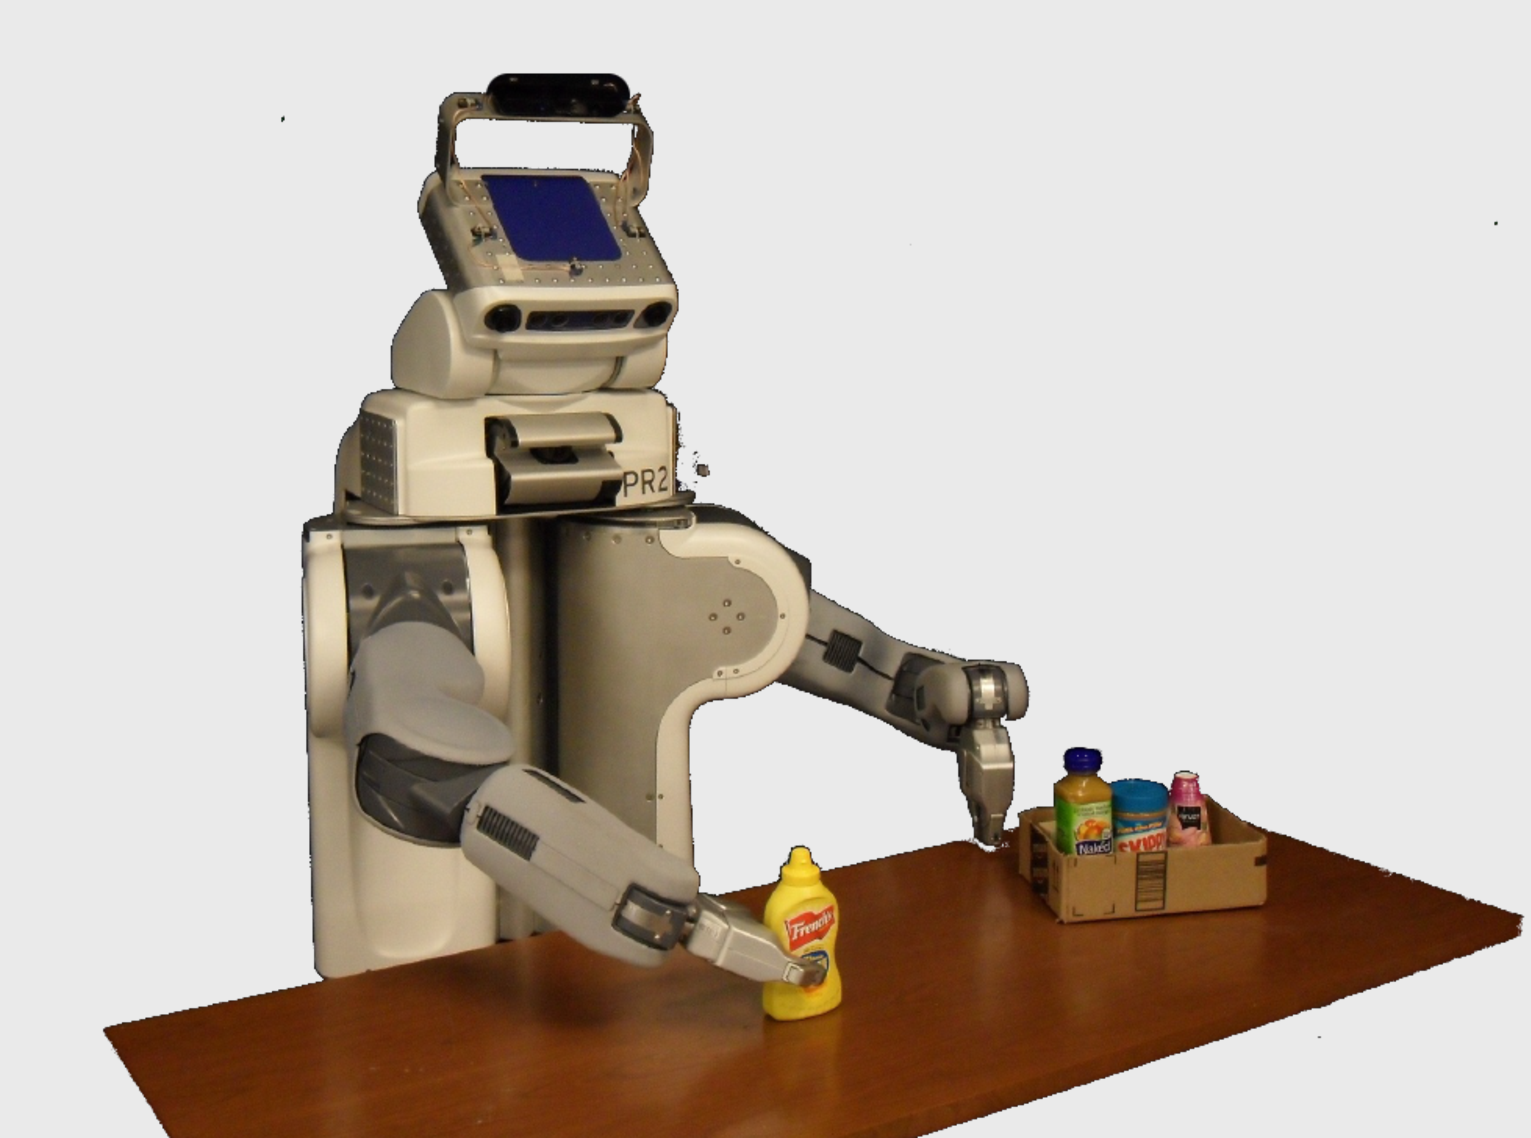
\includegraphics[width=1\textwidth]{Cap1/Figuras/pr2_grasping.pdf}
         \caption{Domestic employment~\cite{pr2robot}.}
         \label{fig:g2}
     \end{subfigure}
    \end{tcolorbox}
    \caption{Robotic grasping in different contexts.}
    \label{fig:most_usual_gripper_forms}
  }%end of resize box      
\end{figure}


In the early days, robotic manipulation was resumed as a context of human teleoperation \cite{bejczy1980sensors}. More recently, it evolved to \ac{PbD} \cite{ferreira2016stereo} and to the beginnings of \ac{LbD} \cite{suleman2011learning} even though the offline programming had been consolidated in the industrial robot programming \cite{de2020adaptpack,castro2020adaptpack}. The first studies focused on the analytical grasping modelling concerning the stability and equilibrium \cite{diziouglu1984mechanics, Nguyen1987_1, Nguyen1987_2, Ponce1995, Li2003}, as well as metrics to evaluate them~\cite{Ferrari, Bicchi2000, Roa2014}. A large number of papers on this topic have been established, achieving success grasping in specific cases. Nonetheless, the complexity rise when more general solutions are pursued: gripper's design and number of fingers~\cite{chen2020active}; previous knowledge of workpieces shape and properties \cite{babin2019stable,babin2019stable,bjornsson2018automated}, e.g., object-agnostic grasping or not; and cluttered or occluded scenes~\cite{d2020study}.

\begin{figure}[h]
\resizebox{.6\textwidth}{!}{%
\begin{tcolorbox}
\centerline{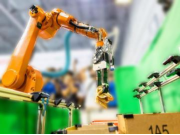
\includegraphics[trim={0cm 0cm 0cm 0cm},clip,width=1\linewidth,angle=0]{Cap1/Figuras/amazon_picking_challenge.pdf}}
\end{tcolorbox}
\caption{Amazon robotic picking challenge winner of 2017 \cite{Zeng2019}. The Amazon robotic picking challenge is an example effort to promote development the warehouse robotic grasping, such as the IROS challenge \cite{iros_challenge}}
\label{fig:}
}
\end{figure}

Subsequently, guided by computer processing and learning algorithms advancements,  works like~\cite{Saxena2008} proved that it is possible to create learning policies to grasping objects, particularly for object-agnostic grasping scenarios. Nowadays, the advent of \ac{DL} and the interesting results achieved in computer vision tasks motivate researchers to explore its capacity to grasp detection \cite{Lenz2015,Redmon2015,Kumra2017,Watson2017,Chu2018,asif2018ensemblenet, Chen2020, Guo2017,Gariepy2019,Mousavian_2019_ICCV,Ghazaei2019,TenPas2017,Chen2019,
Mahler2016,Mahler2017b, Mahler2017d, Mahler2017,Mahler2019,song2020novel}. 

Even with exciting discoveries and results successfully deployed in specific use cases, the robotic grasping still does not have a feasible generalisation solution that comprises the modern industry demands of fast design and easy deployment. It is important to note that, the results assessments standardisation is also a problem. Actually is challenging to study and choose a grasping methodology since several proposals use different results analyses that typically are not in accordance with the application requirements. 


\section{Motivation}
\label{cap1:introduction:motiviation}



%the robotic grasping still does not have a feasible generalisation solution that comprises the modern industry demands of fast design and easy deployment.

Since a complete and generic solution is unreachable until now, there is exists a lack in the deployment of a modular and flexible grasping framework for robots attending real industry demands and a well structured and formalised architecture in which organizes approaches allowing the evaluation and the base to new advancements in science. Therefore, the main Ph.D. question relies in:

\begin{flushright}
``Several approaches achieved interesting robotic grasping results in specific and/or controlled scenarios. However, how to choose and deploy them according to industry demands?"
\end{flushright}

Afterwards, when applying the grasping solution, engineers and researchers still have difficulty comparing the achieved results since the grasping parametrisation and evaluation demand big efforts. Current state-of-art deploy different metrics that, in some cases do not reflex the grasping complexity, which can involve from graspable object detection to stability estimation. Thus, the second PhD question is:

\begin{flushright}
%``How to evaluate a grasping methodology in a standard manner allowing %easy comparison between different techniques?"

``How can a grasping methodology be evaluated in a consistent manner that enables straightforward comparison between various techniques? "
\end{flushright}

%``Several approaches achieved interesting results in specific and/or controlled scenarios. However, how to choose and deploy them according to industry demands?"

%\cred{referenciar  ODS 9: Indústria, Inovação e Infraestruturas}

%-----------------------------------------------------------------------------------------------------------------
\section{Goals}
%-----------------------------------------------------------------------------------------------------------------

Aiming to answer the questions described in Section~\ref{cap1:introduction:motiviation}, the present thesis is summarised into two main objectives:


\begin{itemize_jp}

    \item Design of an innovative modular software architecture able to be hierarchy modified and reconfigured, structured in a pipeline flow which to organise the approaches' studies and evaluation. Therefore, developers can easily integrate new methodologies and end-users can set a pipeline of heuristics according to the task exigences and, choose between the best solution options between methodologies, i.e., the user will just need to pick the method and set its parameters without implementing the methods by self; 

    \item Formalisation and standardisation of the grasping evaluation idea since a grasping problem involves perception, planning, and control. Therefore, a clear standard could improve the methodologies' comparability since each step of the procedure affects the grasping performance. These criteria are applied in state-of-art literature and in the current work.

    %\item Discussion and presentation of the new steps and future works ideas not yet explored: from the academic field to the new challenges of industry 4.0.
    
\end{itemize_jp}

Other specific developments and contributions are highlighted as following:

\begin{itemize_jp}
    \item Discussion and review of state-of-the-art proposals regarding grasping solutions and how they evolved over the years; 
    \item Definition of a grasping dataset standard;
    \item Development of grasping hardware and firmware to support grasping by demonstration applications.
\end{itemize_jp}


%-----------------------------------------------------------------------------------------------------------------
\section{Thesis Organisation}
%-----------------------------------------------------------------------------------------------------------------


The remainder of the thesis is organised as follows: Chapter~\ref{cap2a:background} presents some theoretical background and concepts used in the present thesis. Chapter~\ref{cap2:related_work} shows and discusses the related work, from different grasping representations (since the characterisation is the most important step in any grasping planning approach) to a review of analytical, learning and deep Learning methods. Chapter~\ref{cap3:grasping_eval} presents a grasping evaluation discussion followed by the proposal of formalisation and standardisation of the grasping evaluation idea. Latter, the proposed standard is applied to state-of-art literature. The modular grasping pipeline proposal is described in Chapter~\ref{cap4:modular_grasping_architecture} with its sub-systems and hardware structures. Chapter~\ref{cap5:results} shows the proposal evaluation and test assessments. In the end, Chapter~\ref{cap6:conclusion} presents the conclusion and the future work discussion and suggestions.
 

%-----------------------------------------------------------------------------------------------------------------
